\documentclass[smallextended,natbib]{svjour3}\usepackage[]{graphicx}\usepackage[]{xcolor}
% maxwidth is the original width if it is less than linewidth
% otherwise use linewidth (to make sure the graphics do not exceed the margin)
\makeatletter
\def\maxwidth{ %
  \ifdim\Gin@nat@width>\linewidth
    \linewidth
  \else
    \Gin@nat@width
  \fi
}
\makeatother

\definecolor{fgcolor}{rgb}{0.345, 0.345, 0.345}
\newcommand{\hlnum}[1]{\textcolor[rgb]{0.686,0.059,0.569}{#1}}%
\newcommand{\hlstr}[1]{\textcolor[rgb]{0.192,0.494,0.8}{#1}}%
\newcommand{\hlcom}[1]{\textcolor[rgb]{0.678,0.584,0.686}{\textit{#1}}}%
\newcommand{\hlopt}[1]{\textcolor[rgb]{0,0,0}{#1}}%
\newcommand{\hlstd}[1]{\textcolor[rgb]{0.345,0.345,0.345}{#1}}%
\newcommand{\hlkwa}[1]{\textcolor[rgb]{0.161,0.373,0.58}{\textbf{#1}}}%
\newcommand{\hlkwb}[1]{\textcolor[rgb]{0.69,0.353,0.396}{#1}}%
\newcommand{\hlkwc}[1]{\textcolor[rgb]{0.333,0.667,0.333}{#1}}%
\newcommand{\hlkwd}[1]{\textcolor[rgb]{0.737,0.353,0.396}{\textbf{#1}}}%
\let\hlipl\hlkwb

\usepackage{framed}
\makeatletter
\newenvironment{kframe}{%
 \def\at@end@of@kframe{}%
 \ifinner\ifhmode%
  \def\at@end@of@kframe{\end{minipage}}%
  \begin{minipage}{\columnwidth}%
 \fi\fi%
 \def\FrameCommand##1{\hskip\@totalleftmargin \hskip-\fboxsep
 \colorbox{shadecolor}{##1}\hskip-\fboxsep
     % There is no \\@totalrightmargin, so:
     \hskip-\linewidth \hskip-\@totalleftmargin \hskip\columnwidth}%
 \MakeFramed {\advance\hsize-\width
   \@totalleftmargin\z@ \linewidth\hsize
   \@setminipage}}%
 {\par\unskip\endMakeFramed%
 \at@end@of@kframe}
\makeatother

\definecolor{shadecolor}{rgb}{.97, .97, .97}
\definecolor{messagecolor}{rgb}{0, 0, 0}
\definecolor{warningcolor}{rgb}{1, 0, 1}
\definecolor{errorcolor}{rgb}{1, 0, 0}
\newenvironment{knitrout}{}{} % an empty environment to be redefined in TeX

\usepackage{alltt}  
\smartqed  % flush right qed marks, e.g. at end of proof
\usepackage{graphicx}
\usepackage{array,multirow,graphicx}
\parskip 2mm           
\usepackage{amsmath}
\usepackage{graphicx}
\usepackage{natbib}
\usepackage{url} % not crucial - just used below for the URL 
\usepackage{multirow}
\usepackage{mathtools}
\usepackage{amsfonts}
\usepackage{rotating}
\usepackage{booktabs}
\usepackage{verbatim}
\usepackage{mathrsfs}
\usepackage{hyperref}
\usepackage{pdflscape}
\usepackage{caption}
\usepackage{tablefootnote}
\usepackage{verbatim}
\usepackage{setspace}
\usepackage[utf8]{inputenc}
\usepackage{authblk}
\usepackage{pdfpages}
\usepackage{fancyhdr}

\newcommand{\blind}{0}

\newcommand{\blA}{\mbox{\boldmath {\bf A}}}
\newcommand{\blB}{\mbox{\boldmath {\bf B}}}
\newcommand{\blW}{\mbox{\boldmath {\bf W}}}
\newcommand{\blX}{\mbox{\boldmath {\bf X}}}
\newcommand{\blM}{\mbox{\boldmath {\bf M}}}
\newcommand{\blx}{\mbox{\boldmath {\bf x}}}
\newcommand{\bla}{\mbox{\boldmath {\bf a}}}
\newcommand{\blalpha}{\mbox{\boldmath {\alpha}}}
\IfFileExists{upquote.sty}{\usepackage{upquote}}{}
\begin{document}





\title{Interactive Graphics for Visually Diagnosing Forest Classifiers in R} 


\author{Natalia da Silva \and
        Dianne Cook\and
        Eun-Kyung Lee}

%\authorrunning{Short form of author list} % if too long for running head

\institute{Corresponding author: Natalia da Silva \at
              Instituto de Estadística (IESTA), Universidad de la República, Montevideo, Uruguay.\\
              \email{natalia.dasilva@fcea.edu.uy}\\
              ORCID:0000-0002-6031-7451\\
           \and
          Dianne Cook \at 
          Department of Econometrics and Business Statistics, Monash University, Melbourne, Australia.\\
          \email{dicook@monash.edu}\\
          ORCID:0000-0002-3813-7155\\
          \and
          Eun-Kyung Lee \at
          Department of Statistics, Ewha Womans University, Seoul, South Korea.\\
          \email{lee.eunk@gmail.com}
}


\date{Received: date / Accepted: date}

\maketitle

\begin{abstract}
This article describes structuring data and constructing plots to explore forest classification models interactively. A forest classifier is an example of an ensemble since it is produced by bagging multiple trees. The process of bagging and combining results from multiple trees produces numerous diagnostics which, with interactive graphics, can provide a lot of insight into class structure in high dimensions. Various aspects of models are explored in this article, to assess model complexity, individual model contributions, variable importance and dimension reduction, and uncertainty in prediction associated with individual observations. The ideas are applied to the random forest algorithm and projection pursuit forest but could be more broadly applied to other bagged ensembles helping in the interpretability deficit of these methods. Interactive graphics are built in R using the \texttt{ggplot2}, \texttt{plotly}, and \texttt{shiny} packages.
\keywords{Statistical Visualization \and Interactive Visualization \and Interpretable Machine Learning \and Ensemble Model}
\end{abstract}

\newpage

\section{Introduction}
\label{sec:intro}

The random forest (RF) algorithm~\citep{breiman1996bagging} was one of the first ensemble classifiers developed. It combines the predictions from individual classification and regression trees (CART)~\citep{breiman1984cl} built by bagging observations~\citep{breiman1996bagging} and random predictor sample at each tree node. These produce diagnostics in the form of uncertainty in predictions for each observation, importance of variables for the prediction, predictive error for future samples based on out-of-bag (OOB) case predictions, and similarity of observations based on how often they group together in the trees.

Ensemble classifiers have grown in popularity~\citep{dietterish00, talbot09}, and the basic ideas behind the random forest can be applied to virtually any type of model. The benefits for classification are reduced variability in predictive error, and the suite of diagnostics provides the potential for better understanding the class structure in the high-dimensional data space. The use of visualization on these diagnostics, in association with multivariate data plots, completes the process to better understand the underlying problem.

A conceptual framework for model visualization can be summarized in three strategies: (1) visualize the model in the data space, (2) look at all members of a collection of a model, and (3) explore the complete process of model fitting~\citep{wickham2015visualizing}. The first strategy is to explore how well the model captures the data characteristics (the model in the data space), which contrasts with determining if the model assumptions hold (data in the model space). The second strategy is to look at a group of models instead of only the best model. This strategy can offer a broad understanding of the problem by comparing and contrasting possible models. The last strategy focuses on exploring the process of the model fitting in addition to the end result.

There has been some, but not abundant, research on visualizing classification models.
\cite{urbanek2002exploring} presents interactive tree visualization implemented in the java software called \verb# KLIMT# that includes zooming, selection, multiple views, interactive pruning, and tree construction as well as the interactive analysis of forests of trees using treemaps. \cite{cutler15raft} developed a java package called \verb# RAFT# to visualize a forest classifier, that included variable selection, parallel coordinate plots, heat maps, and scatter plots of some diagnostics. Linking between plots is limited. \cite{quach2012interactive} presents interactive forest visualization using the R package \verb# iPlots eXtreme # \citep{urbanek2011iplots} where several displays are shown in one window with some linking between them available. \cite{Silva2016} describes visualizing components of an ensemble classifier.

This article describes structuring interactive graphics to facilitate visual exploration of ensemble classifiers using RFs and projection pursuit random forests (PPF)~\citep{da2021projection} as examples. The PPF algorithm builds on the projection pursuit tree (PPtree)~\citep{lee2013pptree} algorithm which uses projection pursuit at each tree node to find the best linear combination of variables to separate the classes. Figure \ref{bounds} shows the boundary that would result from a classification tree fitted using the PPtree algorithm (Example from \citep{da2021projection}).

The visualization approach is consistent with the framework in \cite{wickham2015visualizing}, and the implementation is built on the newest interactive graphics available in R \citep{RCore}. The purpose is to provide readily available tools for users to explore and improve ensemble fits and obtain an intuition for the underlying class structure in data. Interactive plots are a key component for model visualization that helps the user see multivariate relationships and be more efficient in model diagnosis. Multiple levels of data are constructed for exploration: observation, model, and ensemble summaries.
The visualization tools presented in this article help open up black-box models and contribute to the interpretability of these methods.



\begin{figure}[!t]
\begin{knitrout}
\definecolor{shadecolor}{rgb}{0.969, 0.969, 0.969}\color{fgcolor}
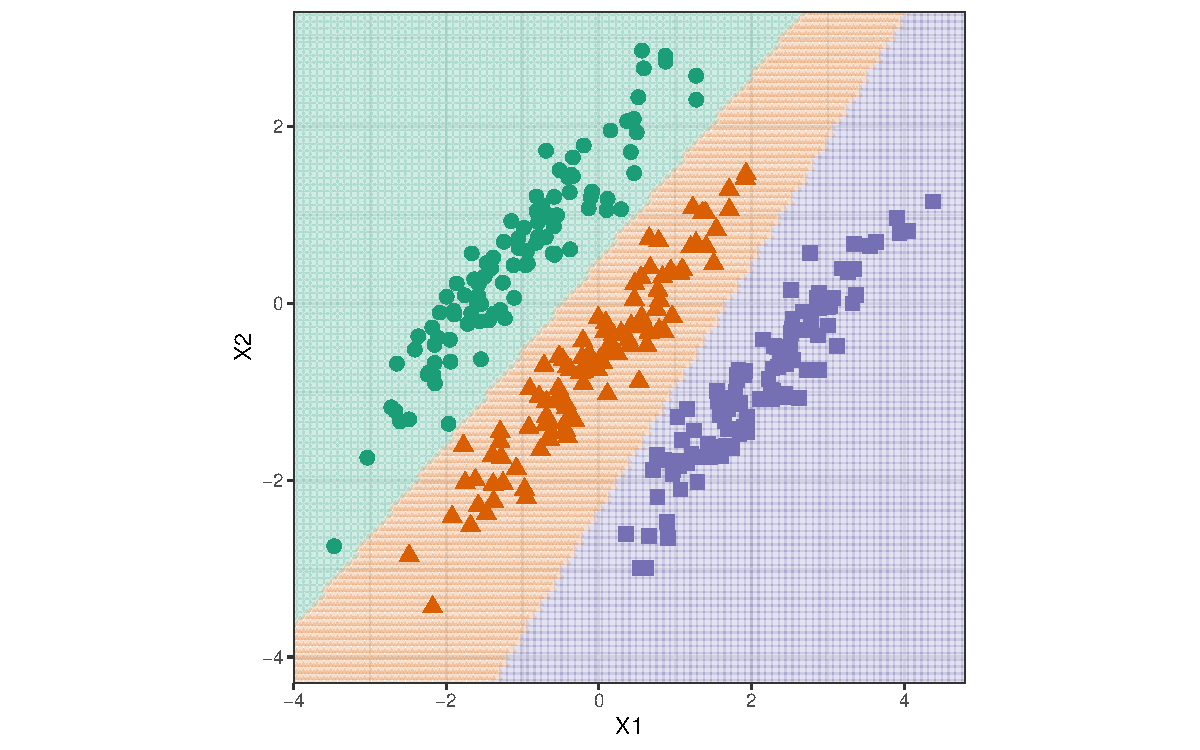
\includegraphics[width=\maxwidth]{boundss-1} 
\end{knitrout}
 \vspace*{-0.3cm}
 \caption{Decision boundaries for PPtree algorithm on 2D simulated data. The partitions generated by PPtree algorithm are oblique to the axis, incorporating the association between the two variables.\label{bounds}}
\end{figure}
Two data sets are used in this paper, crab~\citep{CM74} and fishcatch data~\citep{fishcatch}. To illustrate the mapping of diagnostics to visualization crab data are used because of its simplicity. The second data set is introduced to illustrate the interactive web app which combines the visualizations introduced in this paper and present a more complex problem to explore within the application.

The article is structured as follows.  Section \ref{key} describes the ensemble components to be assessed.  Section \ref{visen} maps the ensemble components to the visual elements. The web app is described in Section \ref{app} and further work is discussed in Section \ref{fur}.

\section{Diagnostics in Forest Classifiers}\label{key}

The diagnostics typically available are:

\begin{itemize} \itemsep 0in
\item {\em \textbf{Out-of-bag error:}} For each model in the ensemble, some cases of the original data are not used. Predicting the response for these cases gives a better estimate for the error of the model with future data. The OOB error rate is a measure for each model that is combined in the ensemble and is used to provide the overall error of the ensemble.\\

\item {\em \textbf{Uncertainty measure for each observation:}} Across individual (classification) models we can compute the proportion of times that a case is predicted to be in each class. If a case is always predicted to be the true class, there is no uncertainty about an observation. Cases that are predicted to be multiple classes, with similar class probabilities, indicate  difficult to classify observations. They may be important by indicating neighborhoods of the data space that would benefit from a more complex model, or simply, measurement errors in the data.\\

\item {\em \textbf{Variable importance:}} Each model uses samples of variables. Thus, the accuracy of the models can be compared when the variable is included or omitted. There are several versions of statistics that use this to provide a measure of the variable importance for prediction.\\

\item {\em \textbf{Similarity measure for pairs of observations:}} In each model, a pair of observations will be either in the same terminal node or not. This is used to compute a proximity matrix. Cluster analysis on this matrix can be used to follow up the classification to assess the original labeling. It may suggest improvements or mistakes in original labels.
\end{itemize}
In addition to these overall ensemble statistics, each individual model has its own diagnostics, measuring error, variables utilized, and class predictions. Visualization will enable the individual models to be examined, relate these to the data and their contribution to the ensemble.

\section{Mapping Ensemble Diagnostics to Visual Components}
\label{visen}

This section describes the mapping of diagnostics to visualizations. These are illustrated using the Australian crabs data~\citep{CM74}. The data has 200 cases, 5 predictors, and 4 classes (combinations of species and sex, BM, BF, OM, and OF). The predictors are: FL (the size of the frontal lobe length, in mm), RW (rear width, in mm), CL (length of mid-line of the carapace, in mm), CW (maximum width of carapace, in mm), BD (depth of the body; for females, measured after displacement of the abdomen, in mm). This is old data, but it provides a good illustration of the visual methods.

\subsection{Individual Models: PPtree}

The PPF is composed of individual projection pursuit trees. PPtree algorithm uses a multi-step approach to fit a multi-class model by finding linear combinations to split on based on projection pursuit algorithm. Two projection pursuit indexes are used to find projections that separate classes,  LDA  \citep{lee2005projection} and PDA \citep{lee2010projection}.

The LDA index is defined as follows:

\begin{equation}
\label{lda}
 \mathbb{I}_{LDA}(\blA) = \left\{
  \begin{array}{l l}
    1-\frac{|\blA^T \blW\blA|}{|\blA^T(\blW+\blB)\blA|} &  \text{for}~|\blA^T(\blW+\blB)\blA|\neq 0\\
    0 &  \text{for}~|\blA^T(\blW+\blB)\blA|= 0
  \end{array} \right.
\end{equation}

\noindent where $p\times q$ matrix $\blA = [\bla_1, \bla_2 , . . . , \bla_q ]$ defines an orthonormal projection from $p$-dimensions onto a $q$-dimensional subspace, $\blB=\sum_{g=1}^G n_g(\bar{\mathbf{x}}_{g}-\bar{\mathbf{x}})(\bar{\mathbf{x}}_{g}-\bar{\mathbf{x}})^{T}$ is the $p\times p$ between-group sum of squares,
$\blW=\sum_{g=1}^{G}\sum_{i\in H_g}(\mathbf{x}_{i}-\bar{\mathbf{x}}_{g})(\mathbf{x}_{i}-\bar{\mathbf{x}}_{g})^T$ is the $p\times p$  within-group sum of squares where $H_g=\{i| y_i = g, i = 1, ..., n\}$, $\bar{\mathbf{x}}_{g}$ is the group mean vector and $\bar{\mathbf{x}}$ the overall mean vector. If the LDA index value is high, there is a large difference between classes.

The PDA index is useful when $n$ is small relative to $p$ and when the variables are highly correlated. In these situations the maximum likelihood variance-covariance matrix estimator will be close to singular, affecting the inverse calculation. The PDA index adjusts the variance-covariance matrix calculation, as follows:


\begin{equation}
\mathbb{I}_{PDA}(\blA,\lambda)=1-\frac{|\blA^T \blW_{PDA}(\lambda)\blA|}{|\blA^T (\blW_{PDA}(\lambda)+\blB) \blA|}
\end{equation}

\noindent where the notation is analogous to the LDA index, with the addition of $\lambda \in [0,1)$ which is a shrinkage parameter, and a different within group sum of squares, $\blW_{PDA}(\lambda)=\mbox{diag}(\blW)+(1-\lambda)\mbox{offdiag}(\blW)$.

Figure \ref{pptreeviz1} shows a visual ensemble of plots of a tree model on the crab data using LDA index (Equation \ref{lda}) and two variables in each node split. There are three nodes for the four class problem. The nodes of this tree are based on projections of the data and their coefficients form the building block to calculate the variable importance. The density plot displays the data projection at each node, and the mosaic plot shows the confusion matrix for the nodes.
The package \verb#PPtreeViz# provides visual tools to diagnose a PPtree model. The PPF builds on these and modifies a little. The PPtree model is simpler than a regular classification tree because the classes are mostly separated by combinations of variables -- just three projections are needed to see the differences between the four classes.

\begin{figure}[hbpt]
\centering
\begin{knitrout}
\definecolor{shadecolor}{rgb}{0.969, 0.969, 0.969}\color{fgcolor}
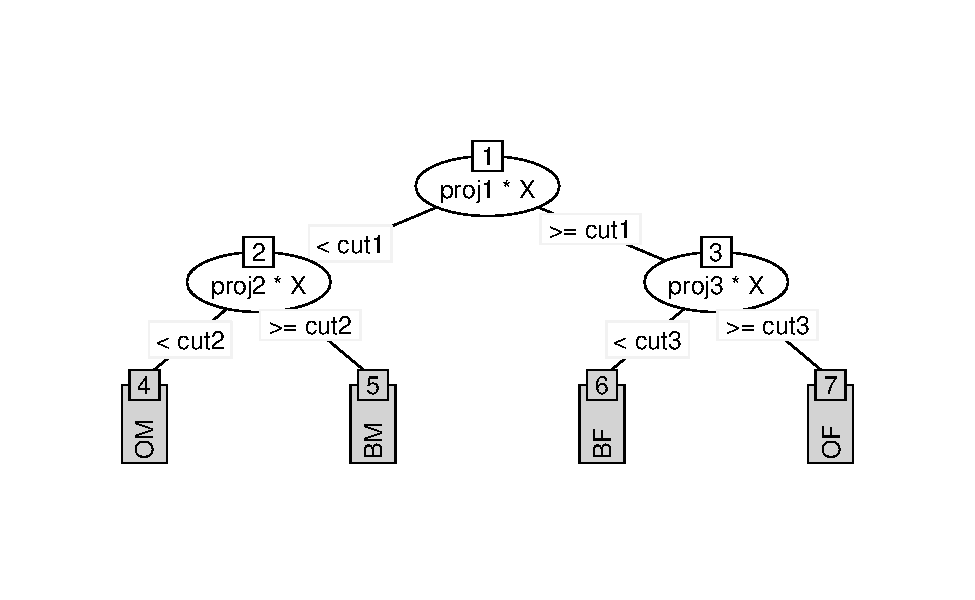
\includegraphics[width=\maxwidth]{trcomb-1} 

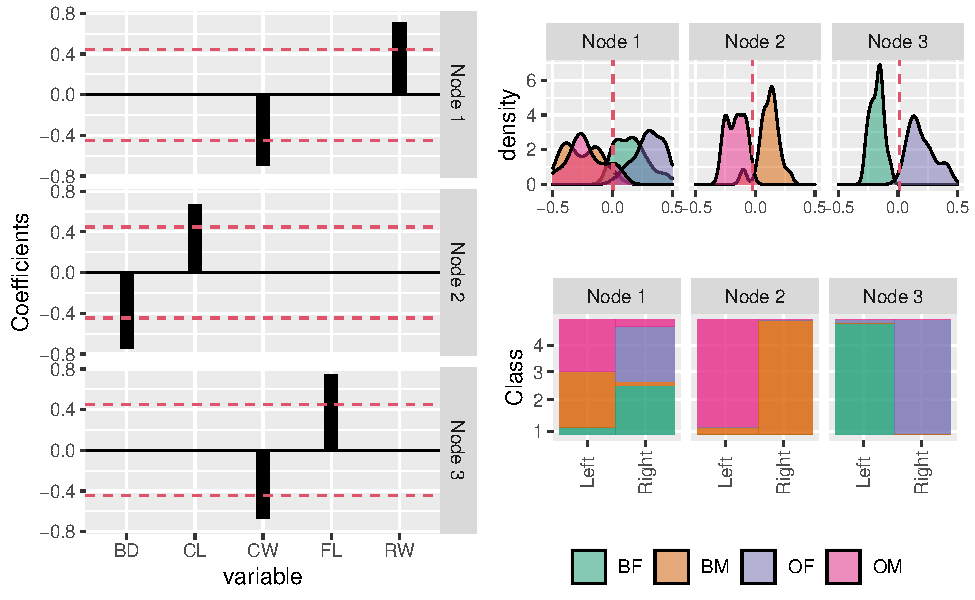
\includegraphics[width=\maxwidth]{trcomb-2} 
\end{knitrout}
\caption{Visualizing the PPtree model of the crab data. The tree has three nodes (top). The density plots show the data projections at each node, colored by group (middle). The dashed vertical red line indicates the split value of each node. Node 1 separates the sexes. Node 2 separates males from species and node 3 separates females from species. Mosaic plots of the confusion table for each split (bottom). Node 1 shows the clear split of sexes, with a small number of misclassifications. Node 2 where BM are separated from OM with a small number of misclassifications. Node 3 where BF are separated from OF, almost perfect classification.\label{pptreeviz1}}
\end{figure}

\subsection{Variable Importance}

The PPF algorithm calculates variable importance in three ways: permuted importance using accuracy,  and two importance measures based on projection coefficients on standardized variables.

The first importance measure is comparable with the measure defined in the classical random forest algorithm. Importance variable is computed based on the OOB cases for the tree $k\;\;(O_k)$ for each $j$ predictor variable.
Permuted importance of the variable $j$ in the tree $k$ is defined in Equation \ref{vi1}.

\begin{equation}
VI^{(1)} _{jk} = \frac{\sum_{i \in O_k } I(y_i=\hat y_{ik})-I(y_i=\tilde y_{ik})}{\# O_k}
\label{vi1}
\end{equation}

\noindent where $\hat y_{ik}$ is the predicted class for the observation $i$ in the tree $k$, and $\tilde y_{ik}$ is the predicted class for the observation $i$ in the tree $k$ after permuting the values for variable $j$. The global permuted importance measure is the average importance over all the trees in the forest. This measure is based on comparing the accuracy of classifying OOB observations using the true class with permuted (nonsense) classes.

The coefficients of each projection are examined to define the other two importance measures. If the variables have been standardized, the magnitude of these values indicates importance. For a single PPtree the variable importance is computed by a weighted sum of the absolute values of the coefficients across nodes, then the weights take the number of classes in each node into account~\citep{lee2013pptree}.

The global variable importance in a PPforest then can be defined in different ways. One way is to average the variable importance from each PPtree across all the trees in the forest (Equation \ref{vi2}).

\begin{equation}
VI^{(2)}_j=\frac{1}{B}\sum_{k=1}^B \sum_{s= 1}^{S}\frac{|a^{**}_{sjk}|}{G_s }
\label{vi2}
\end{equation}

\noindent where $a^{**}_{sjk}$ is the projected coefficient for node $s$ and variable $j$ in the $k^{th}$ PPtree, and $S$ is the total number of node partitions in the $k^{th}$ tree. Note that $\sum_{s= 1}^{S}\frac{|a^{**}_{sjk}|}{G_s }$ is the importance of the variable $j$ in the PPtree $k$.

Alternatively, it can be computed as a weighted mean of the absolute value of the projection coefficients across all nodes in every tree as shown in Equation \ref{vi3}.

\begin{equation}
VI^{(3)}_j=\frac{1}{B}\frac{1}{G-1}\sum_{k=1}^B\sum_{s = 1}^{S} (1-e_k) I_{sjk}|a^{**}_{sjk}|
\label{vi3}
\end{equation}

\noindent where $e_k$ is the OOB error rate of tree $k$, $I_{sjk}$ is the projection pursuit index value of node $s$ ~\citep{da2021projection}.

Figure \ref{impotree} shows the absolute projection coefficient of the top three nodes for all the trees in a forest model. This information is displayed by a side-by-side jittered dot plot. The red dots correspond to the absolute coefficient values for the tree model of Figure \ref{pptreeviz1}. The forest was built using random samples of two variables for each node, hence there are two coefficients for each node. At node 1 uses CW and RW with similar contribution. The scatterplot at right shows these two variables and the resulting boundary between groups that this would produce. Node 2 uses BD and CL where BD contributes the most to the separation. The plot in the right shows the boundary that is induced. Node 3 uses CW and FL with an even contribution by the two variables. Alternative visualizations for the importance variable plot can be considered, for example violin plots or boxplots however, the side-by-side jittered dot plot was preferred since presents individual details on importance measure distribution.

For each tree in the forest, different decision rules are defined; the resulting boundaries on the previous plots are based on Rule 1 $= \frac{m_1}{2} + \frac{m_2}{2} $, where $m_1$ and $m_2$ are the mean of the left and right groups at each node.

\begin{figure}[hbpt]
\centering
\begin{knitrout}
\definecolor{shadecolor}{rgb}{0.969, 0.969, 0.969}\color{fgcolor}
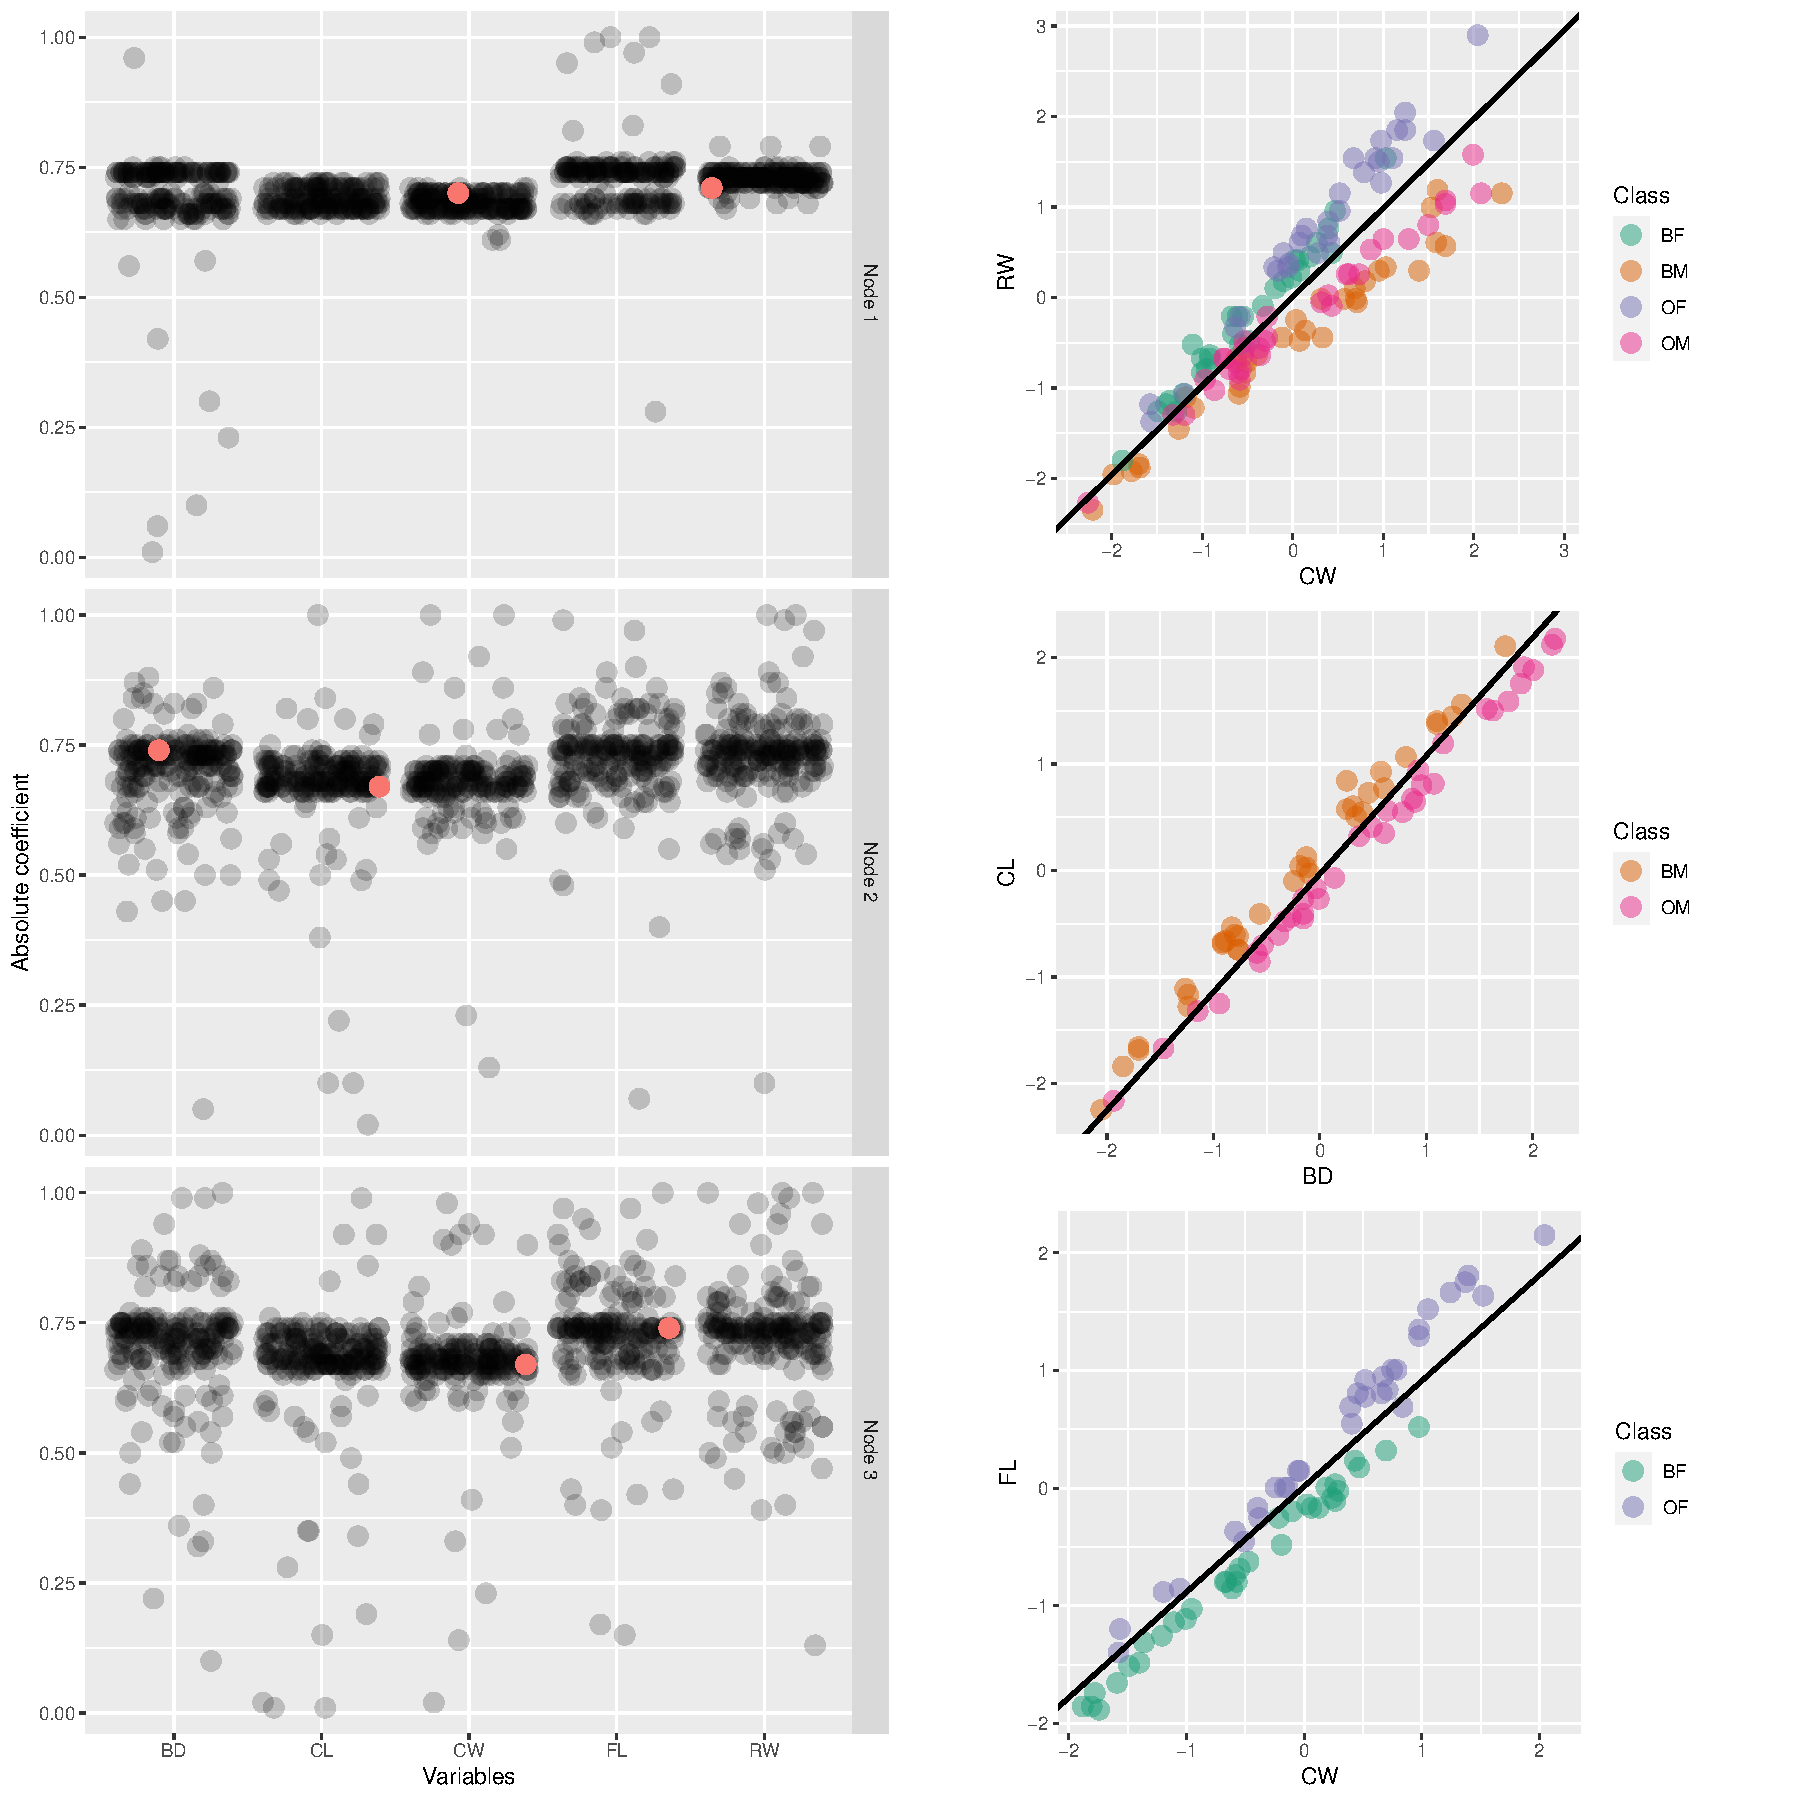
\includegraphics[width=\maxwidth]{treenode-1} 
\end{knitrout}
\caption{Visualizing the variable importance of all the trees in the forest, for three nodes. Every particular node of each tree has an importance value for the corresponding variable. The values for the whole forest are displayed using a side-by-side jittered dot plot. The importance values are the absolute values of the projection coefficients. The red points correspond to these values for the tree shown in Figure \ref{pptreeviz1}. Two variables are randomly selected at each node for creating the best projection, and split. The plots at right show the variables used and the split made at each of the nodes of this tree.  \label{impotree}}
\end{figure}

\newpage

\subsection{Similarity of Cases}

For each tree, every pair of observations can be in the same terminal node or not. Tallying this up across all trees in a forest gives the proximity matrix, an $n\times n$ matrix of the proportion of trees that the pair share a terminal node. It can be considered as a similarity matrix.

Multidimensional scaling (MDS) is used to reduce the dimension of this matrix, to view the similarity between observations ~\citep{kruskal1964multidimensional}. MDS transforms the dataset into a low-dimensional space where the distances are approximately the same as in the full $n$ dimensions. With $G$ groups, the low-dimensional space should be no more than $G-1$ dimensions. Figure \ref{prox1} shows the MDS plots for the three dimensional space induced by the four groups of the crab data. Color indicates the true species and sex. For this data, two dimensions are enough to see the four groups separated quite well. Some crabs are clearly more similar to a different group, especially in examining the sex differences. MDS is included in the interactive web app presented in Section \ref{app}.


\begin{figure}[hbpt]
\centering
\begin{knitrout}
\definecolor{shadecolor}{rgb}{0.969, 0.969, 0.969}\color{fgcolor}
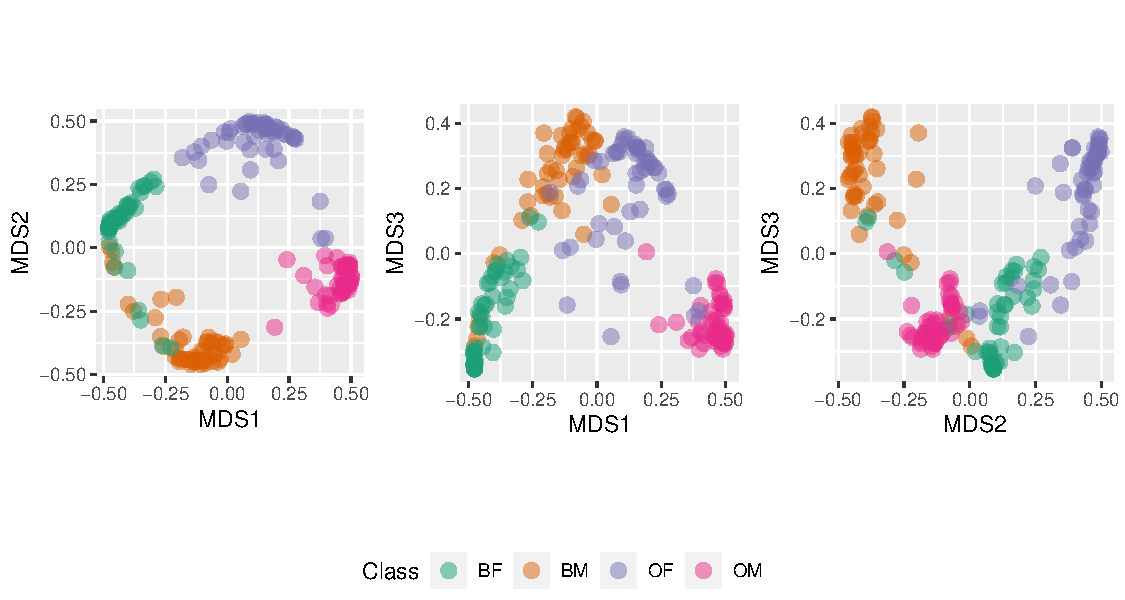
\includegraphics[width=\maxwidth]{mds-1} 
\end{knitrout}
\caption{Examining similarity between cases, using pairwise plots of multidimensional scaling into a three-dimensional space. It can be seen that most cases are grouped closely with their class, and particularly that the two species are distinct. There is more confusion of cases between the sexes. \label{prox1}}
\end{figure}


\subsection{Uncertainty of Cases}

The vote matrix ($n \times G$) contains the proportion of times each observation was classified to each class while OOB. Two approaches to visualize the vote matrix information are used.

A ternary plot is a triangular diagram used to display compositional data with three components. More generally, compositional data can have any number of components, say $p$, and hence is constrained to a $(p-1)$ dimensional simplex in $p$-space. The vote matrix is an example of compositional data with $G$ components.

With G classes, the ternary plot idea is generalized to a $(G-1)- dimensional$ simplex~\citep{sutherland2000orca, schloerke}. This is one of the approaches used to visualize the vote matrix and it is included in the interactive web app presented in Section \ref{app}.

For the crab data, $G=4$ and the generalized ternary plot will be a tetrahedron. Figure \ref{tetra} shows the tetrahedron structure for the crab vote matrix shown in three pairwise views. With well-separated classes, the colored points will each concentrate into one of the vertices. This is close but not perfect, indicating some crabs are commonly incorrectly classified. The \verb#tourr# package~\citep{wickham2011tourr}, tour methods for multivariate data visualization, can be used to view the animated version available for this example in  \url{https://vimeo.com/170522736}.


\begin{figure}[hbpt]
\centering
\begin{knitrout}
\definecolor{shadecolor}{rgb}{0.969, 0.969, 0.969}\color{fgcolor}
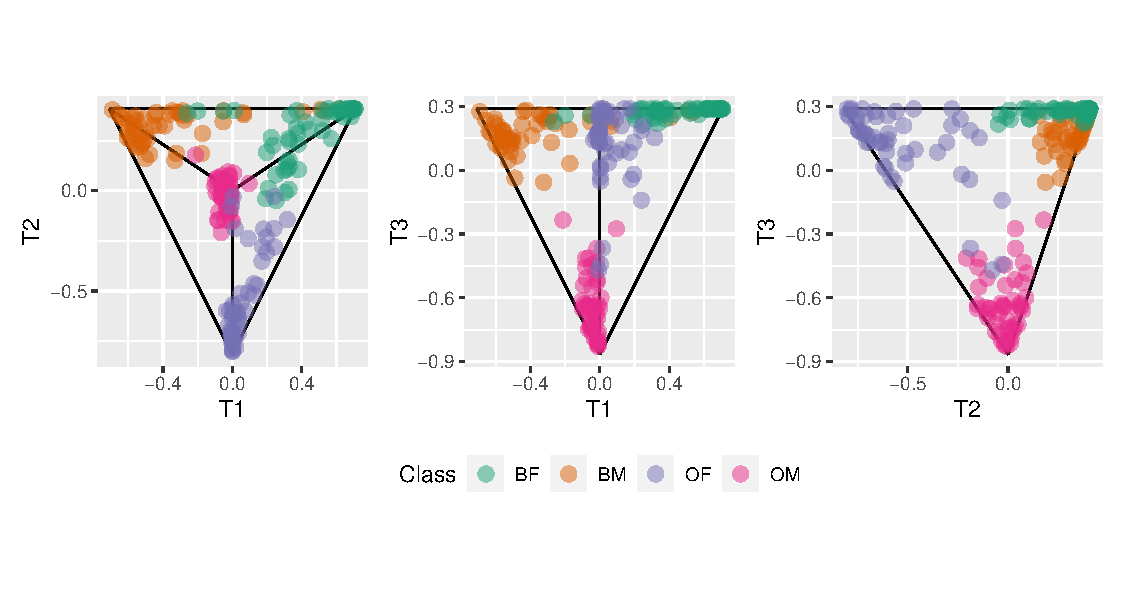
\includegraphics[width=\maxwidth]{ternary-1} 
\end{knitrout}
\caption{Generalized ternary plot ((G-1) dimensional simplex, in this case a tetrahedron) representation of the vote matrix for four classes. The tetrahedron is shown pairwise. Each point corresponds to one observation and color is the true class. This is close but not a perfect classification since the colors are concentrated in the corners and there are some mixed colors in each corner.}
\label{tetra}
\end{figure}

Because visualizing the vote matrix with a $(G-1)$ dimensional tetrahedron requires dynamic graphics, a low-dimensional option is also provided. For each class, every individual case has a value between 0-1. A side-by-side jittered dotplot is used for the display, where the class is displayed on one axis and proportion is displayed on the other. For each dotplot, the ideal arrangement is that points are concentrated at 0 or 1 and only at 1 for their true class. This data is close to the ideal but not perfect, e.g. there are a few BM crabs (orange) that are frequently predicted to be BF (green), and a few BF crabs predicted to be another class.

\begin{figure}[hbpt]
\centering
\begin{knitrout}
\definecolor{shadecolor}{rgb}{0.969, 0.969, 0.969}\color{fgcolor}
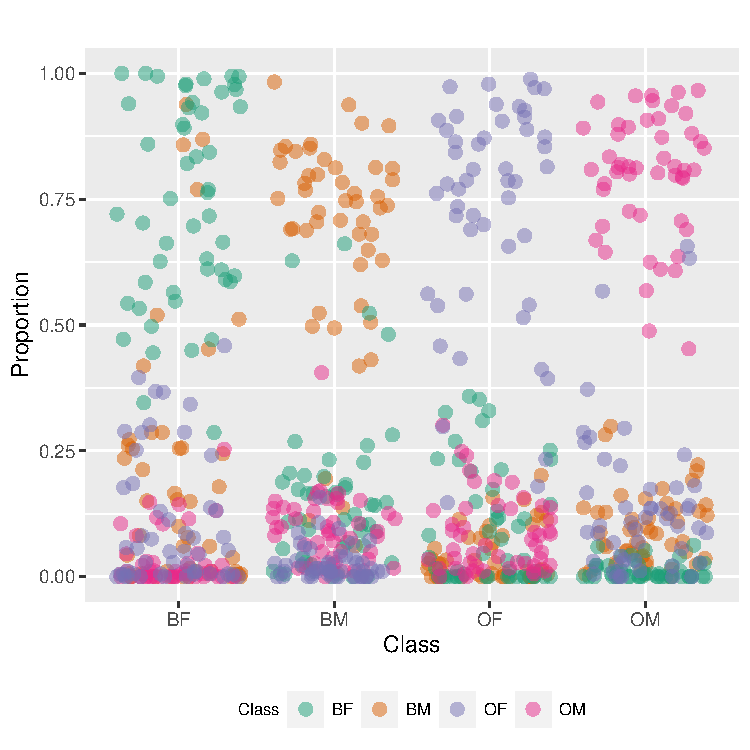
\includegraphics[width=\maxwidth]{side-1} 
\end{knitrout}
\caption{Another representation of the vote matrix, as a jittered side-by-side dotplot. It is not as elegant as the ternary plot, but it is useful because it places focus on each group. Each dotplot shows the proportion of times the case was predicted into the group, with 1 indicating that the case was always predicted to the group and 0 being never. On each dotplot, a single color dominates the top, indicating fairly clear distinctions between classes. Crabs from the B species, both male and female, have more uncertainty in predictions, as seen by more crabs from other classes having higher vote proportions than is seen in the O species.}
\label{sideby}
\end{figure}
 
\section{Interactive Web App }\label{app}

 Interaction is added to the plots described in Section \ref{visen} as well as other plots, which are organized into an interactive web app using \verb#shiny#~\citep{chang11shiny, wickham2021mastering} for exploring the ensemble model. The app is organized into three tabs: individual cases; models; and performance comparison, to provide a model diagnostic tool. Interaction is provided as mouse-over labeling, mouse-click selection and brushing, with results linked across multiple plots. The app takes advantage of new tools provided in the \verb#plotly# package ~\citep{plotly,sievert2020interactive}, developed as a part of Sievert's PhD thesis research~\citep{sievertthesis}.

The \verb#plotly# functions directly translate a static \verb#ggplot2# object by extracting information and storing it in JavaScript Object Notation (JSON). This information is passed as input to a javascript function to produce a web graphic.  Interactions in a single display and links between different graphics are two key tasks an interactive visualization should accomplish~\citep{xie2014reactive}.

As \cite{sievert2020interactive} describes, one of the biggest difficulties when it comes to the app is managing linking between plots (also called a widget in the plotly documentation) requiring careful data structure management. Each plot has its own data structure and interaction. Putting them into the structure of a shiny app facilitates access to the widget data and coordinates selections across multiple plots.

To illustrate the shiny app characteristics, a different dataset (fishcatch) are used which presents a more challenging classification problem and then more interesting results to explore the app. The fishcatch dataset~\citep{fishcatch} contains 159 observations, with 6 physical measurement variables, and  7 types of fish, all caught from the same lake (Laengelmavesi) near Tampere in Finland. There are 35 bream, 11 parkki, 56 perch, 17 pike, 20 roach, 14 smelt and 6 whitewish. The shiny app showing fishcatch data can be accessed at \url{https://natydasilva.shinyapps.io/shinyppforest}.

\subsection{Individual Cases}

This tab is designed to examine uncertainty in the classification of observations and to explore the similarity between pairs of observations. The data feeding the display is an $n\times p$ data frame; containing the original data; the model statistics generated from the full $n\times G$ vote matrix along with its generalized ternary coordinates; and the first two MDS projections of the proximity matrix.

The plots in the tab are (1) a parallel coordinate plot (PCP) of the data, (2) the MDS display of the proximity matrix, (3) side-by-side jittered dotplot, and (4) generalized ternary plot of the vote matrix. Each of these plots are interactive in the sense that each one presents individual interactions (mouse-over) and they are linked so that selections in one display are propagated to other plots (clicking and selecting).

The diagram in Figure \ref{tab1diag} illustrates the data pipeline \citep{BAHM88,wickham2009plumbing} for the interactive graphics in the case level tab.
\begin{figure}[hbpt]
\centering
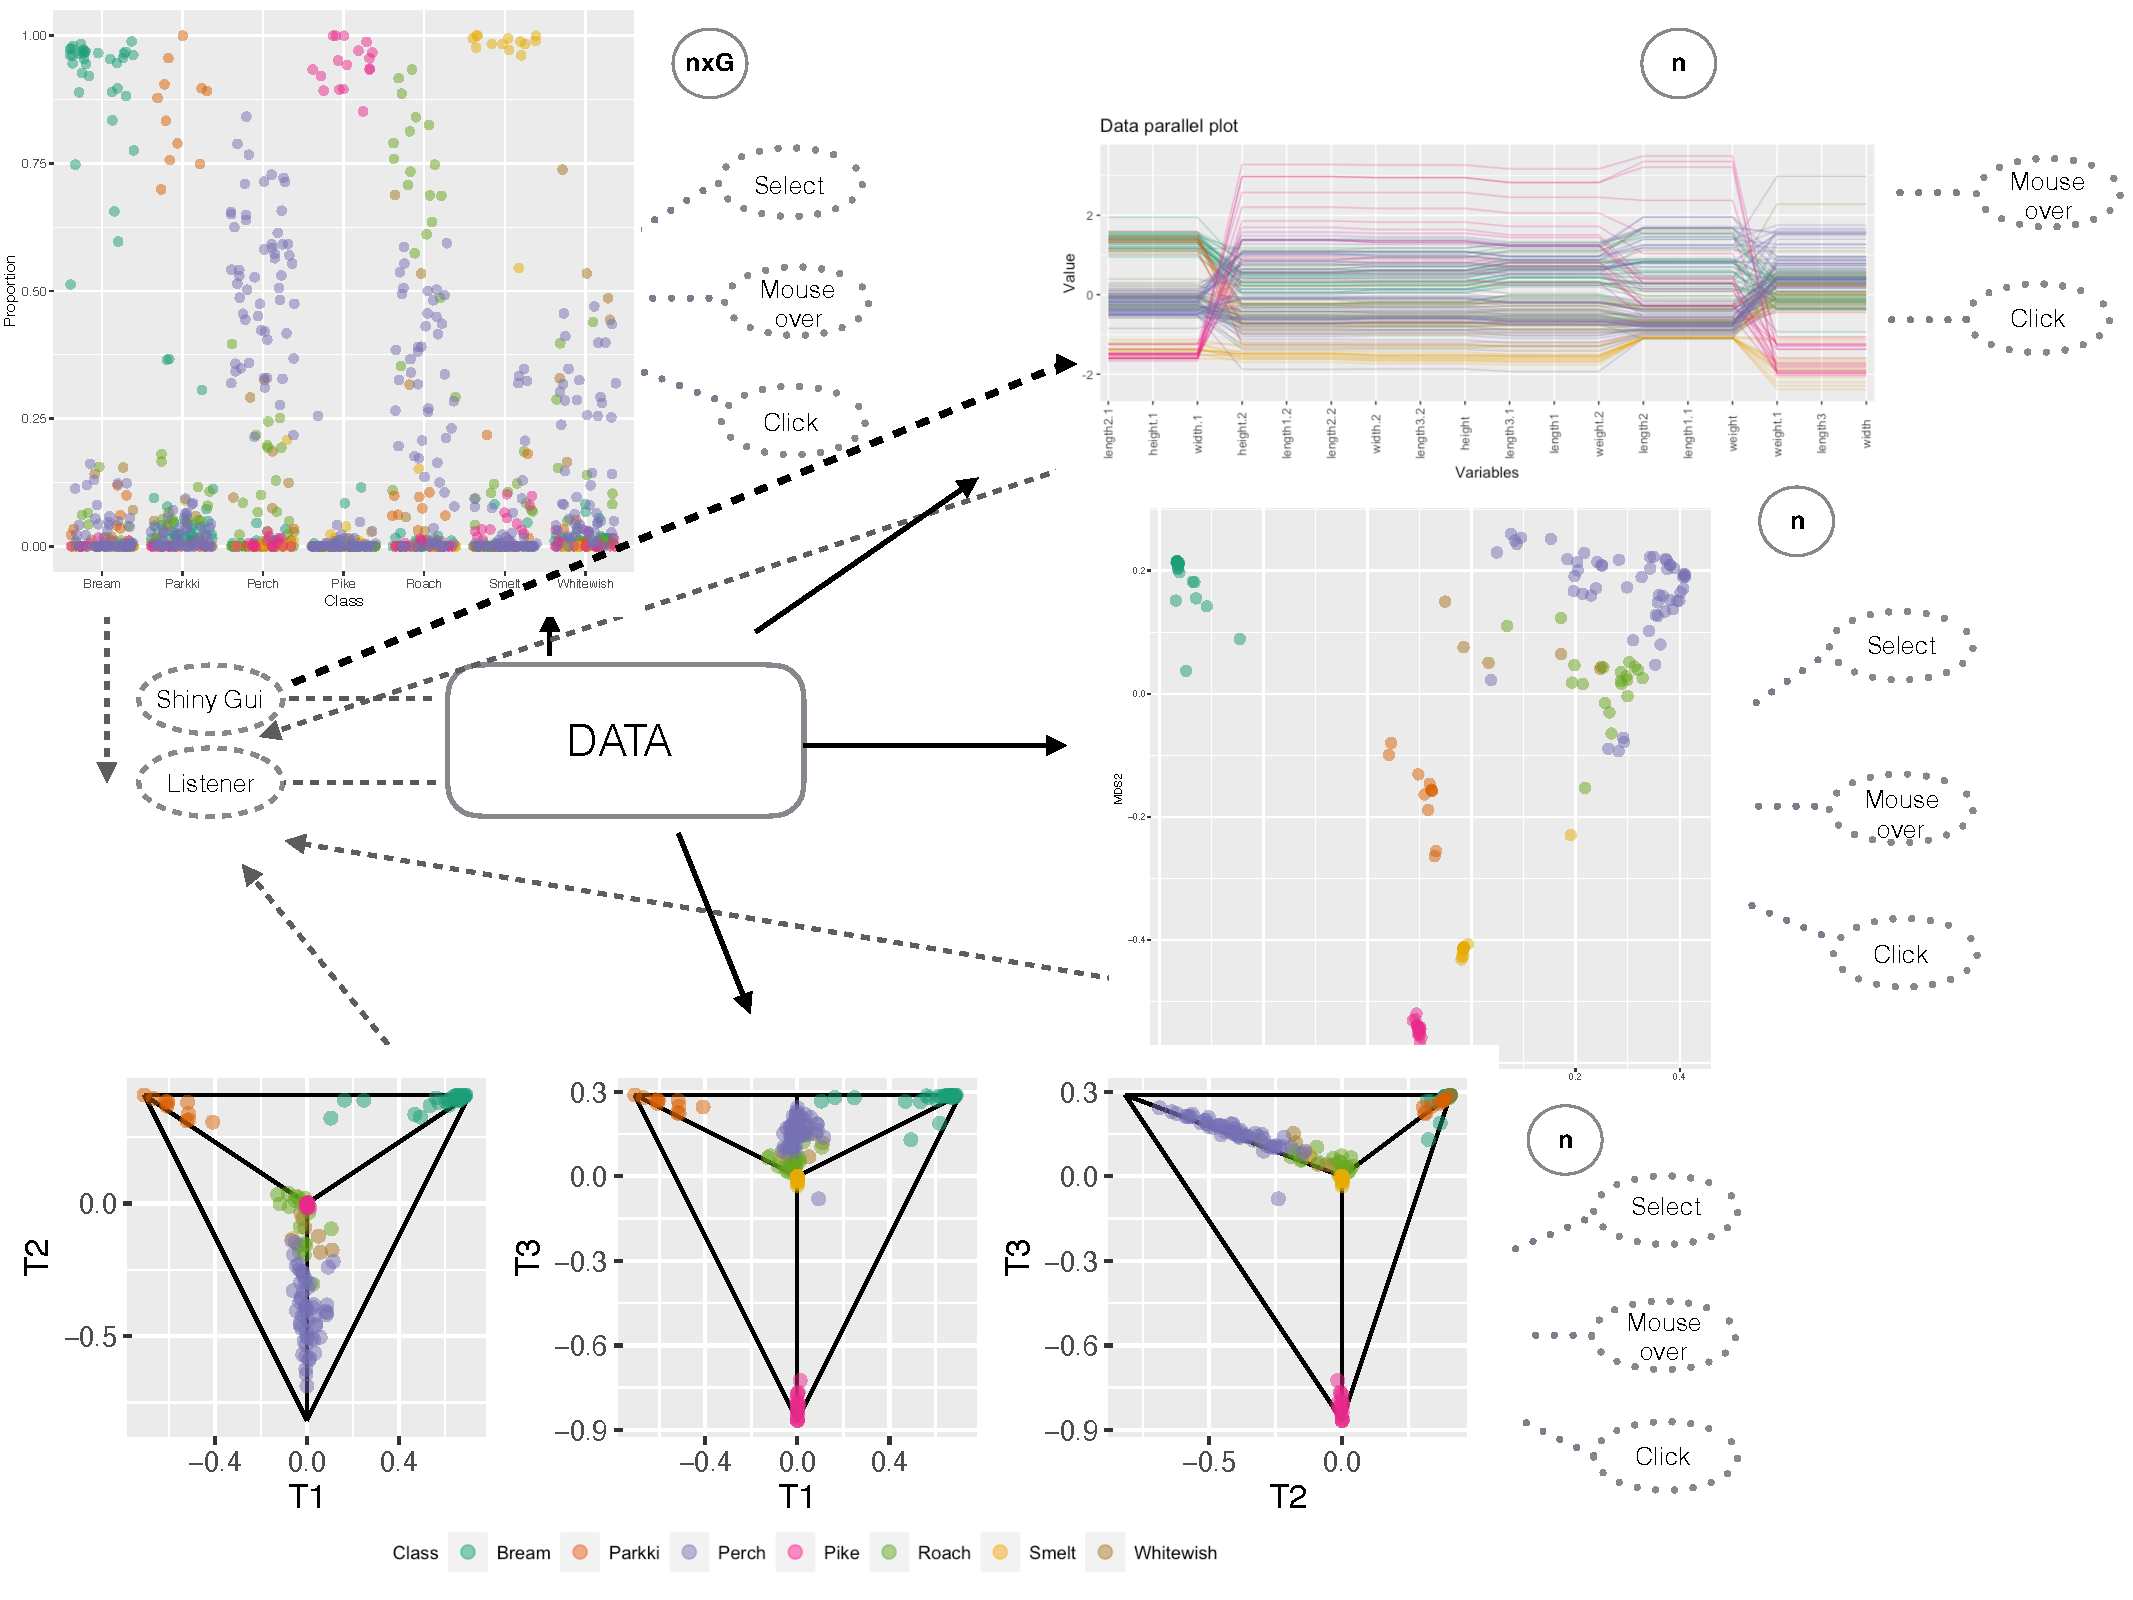
\includegraphics[width=1\linewidth]{fishT1.pdf}
\caption{Schematic diagram illustrating the interactivity in and between plots for individual level exploration panel of the web app. From the data, the four plots are generated. Each plot has a listener attached which collects user actions. When a user selects a point or line in any of the displays, it makes a change in the data which propagates updates to each of the plots.}
\label{tab1diag}
\end{figure}
Solid lines indicate notifications from the source data to the plots, and dashed lines indicate notification of user action on the plot, which notifies the data source of actions to take. The data table is a reactive object that has a listener associated with it. Each of the plots is reactive and has numerous listeners. When users make selections on a plot, either by clicking or group selection, a change to the data is made in terms of an update on the selected cases. This invokes a note to other plots to re-draw themselves. The linking between plots is effectively one-to-one, based on the row ID of the data. The side-by-side jittered dotplot has $n\times G$ points, but selection can only be done within a dotplot. Selecting in one of the dotplots notifies the data table of the selection which triggers a re-draw of the other dotplots. Mouseovers on the plot pull additional information about the point or line under the cursor but do not link between plots.

Figure \ref{tab1} shows the arrangement of plots in this first tab (the case level tab). This selection of plots enables aspects of the model, relating to performance for individual cases, to be examined in the data space. The data plot is an essential element following the {\em model-in-the-data-space} philosophy of \citet{wickham2015visualizing}. The choice was made to use a parallel coordinate plot because it provides a space-efficient display of the data. Alternatives include the tour, a dynamic plot, or a scatterplot matrix. Theoretically, either of these could be substituted or added.
Parallel coordinate plots are useful to visualize multivariate numerical data. As is shown in the first plot in Figure \ref{tab1}, in a PCP each variable is placed equidistant and perpendicular to the x-axis, on the y-axis the values for each variable are standardized to easily compare them. Each observation is represented as a line connected across  all the variables. In a PCP many variables can be compared together and seeing the relationships between them, identify and characterize groups of observations. The features can be ordered so that there are not too many lines intersecting resulting in an unreadable chart \citep{inselberg2009parallel}.
Two alternatives can be selected in shiny to draw the parallel coordinate plot: parallel or enhanced. Parallel draws the classic PCP and enhanced draws a modified version where variables are repeated \citep{hurley2011eulerian}. Because reading a PCP is really only possible for neighboring variables, the variables are repeated so that all variable pairs are shown next to each other once.

\begin{figure}[hbpt]
\centering
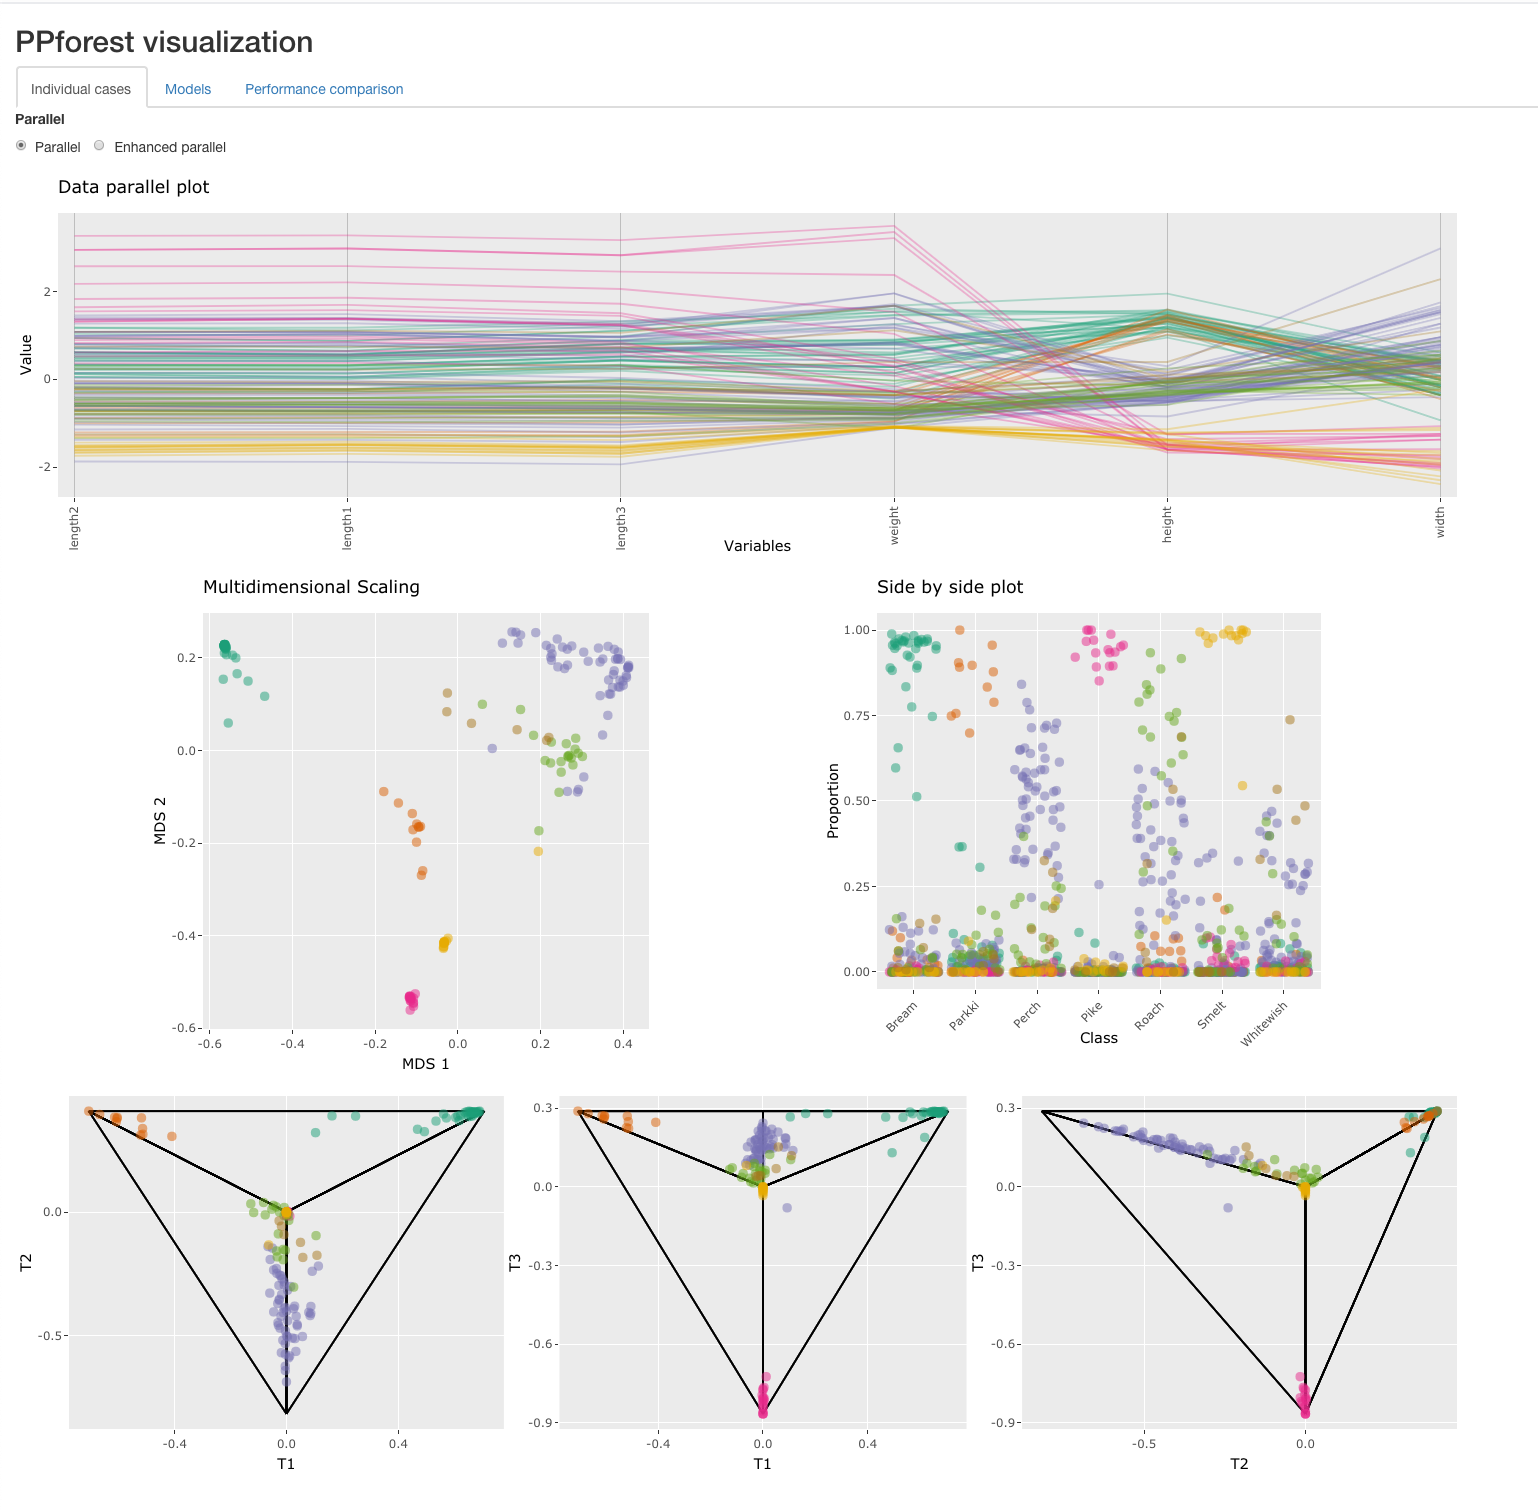
\includegraphics[width=1.05\linewidth]{fish11.png}
\caption{Entry page for the web app, focusing on examining cases, in terms of similarity and uncertainty. The top plot shows the data, the remaining plots show similarity of cases and uncertainty in predictions. All of the plots are linked so that selecting elements of one will generate changes in the others. \label{tab1}}
\end{figure}

Figure \ref{tab1comp} shows the arrangement of plots in this first tab for selected points to illustrate how the tab works. In the MDS plot, the yellow points (smelt) which are grouped were selected, in the parallel plot it is clear all these observations are similar with small values in all the variables and small variability. These are easy points to classify for the model, in the side-by-side jittered dot plot all these points have a   probability of being classified as the correct class (smelt) close to one, and in the ternary plot, all these points are concentrated in the vertices.


\begin{figure}[hbpt]
\centering
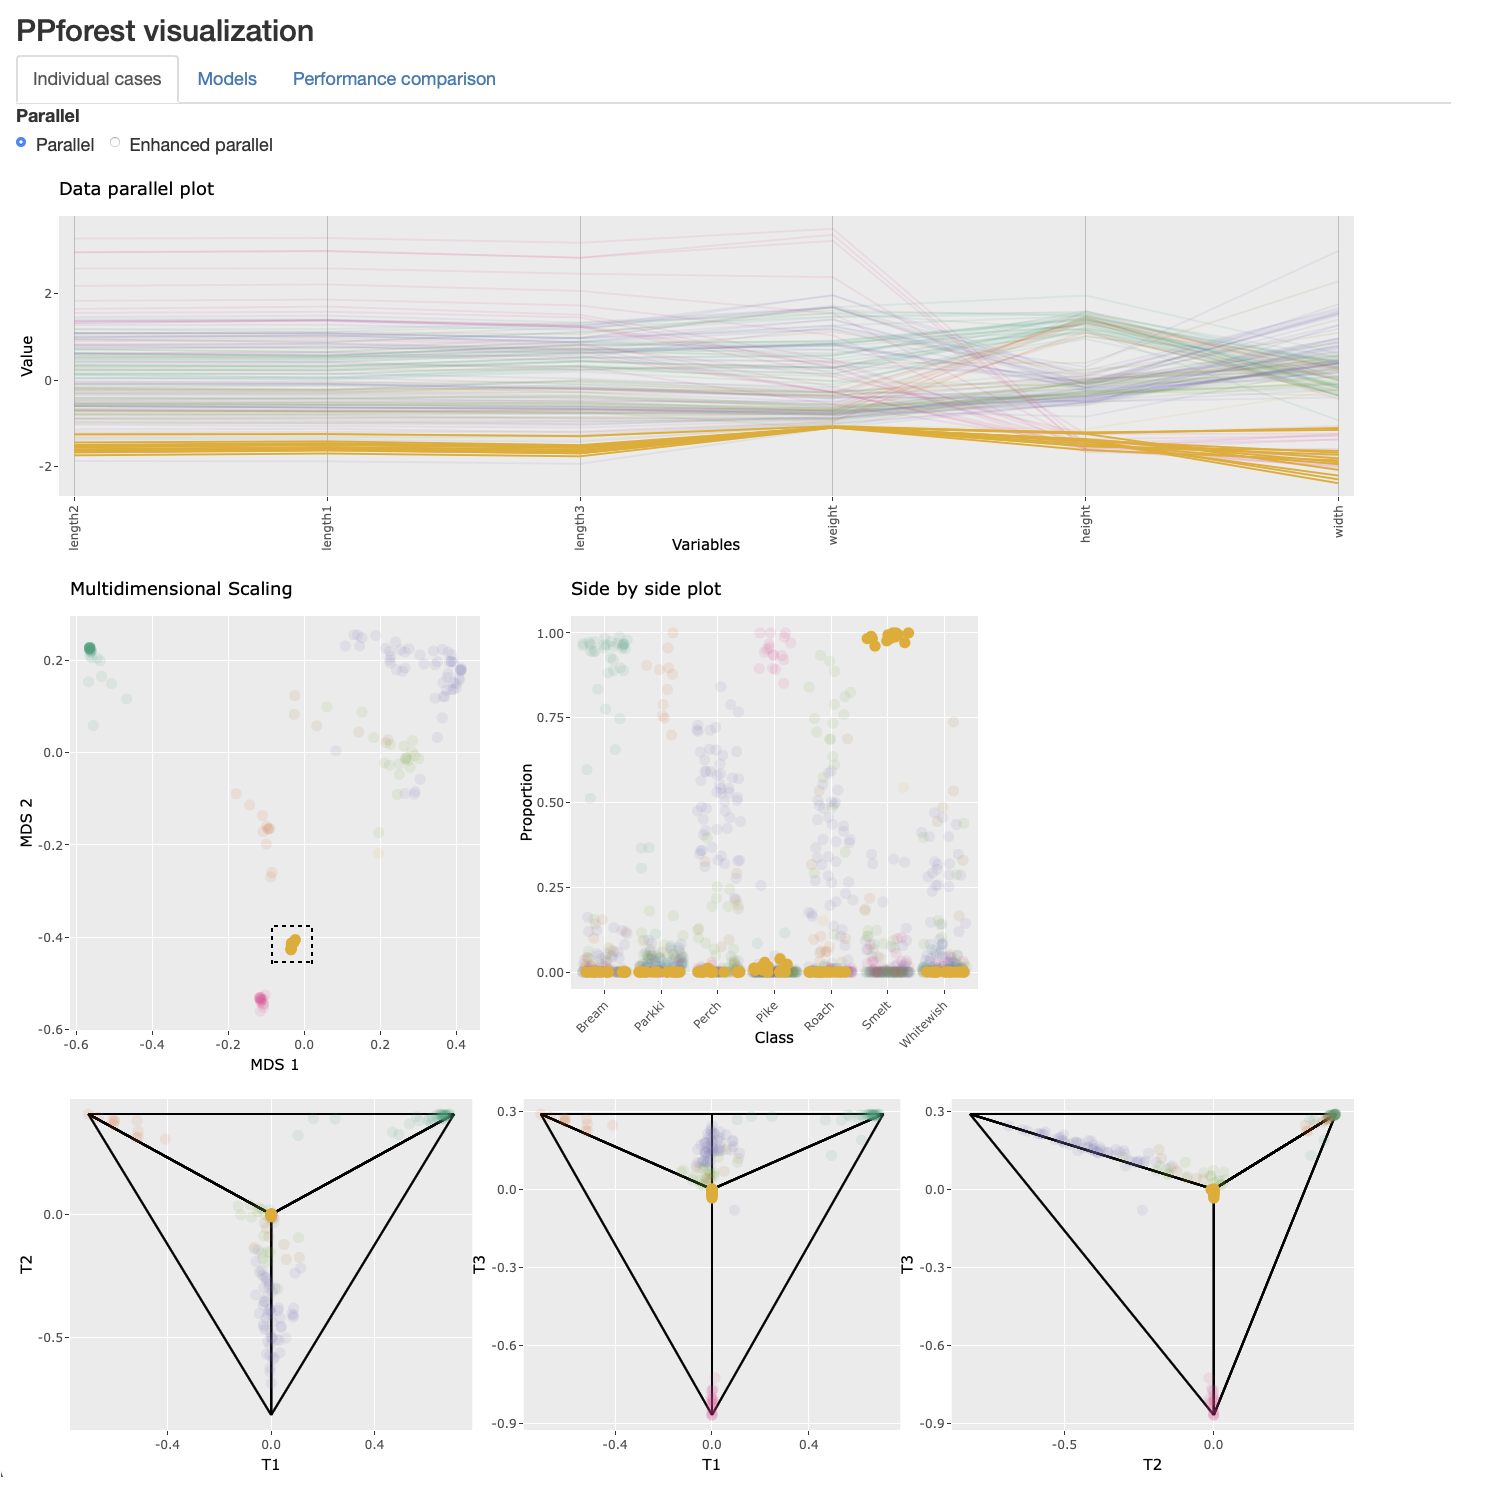
\includegraphics[width=1.1\linewidth]{tab1com2.png}
\caption{Entry page for the web app, focusing on examining cases, for selected points.  \label{tab1comp}}
\end{figure}

\subsection{Models}

This second tab in the app focuses on teasing apart the forest to examine the qualities of each tree. For each tree, information on the variable importance, the projections used at each node, and the OOB error is available. The data feeding into this tab is a list of models along with the original data frame.
The tree ID is displayed when we mouse over the jittered side-by-side plot. This information is useful because, based on the accuracy, some trees could be removed from the forest outside of the app.

Figure \ref{tab2} is a screenshot of the models tab. There are five plots, with varying levels of interaction: (1) a boxplot of OOB error for all trees including the data as jittered points, (2) a jittered side-by-side dotplot showing variable importance for the top three nodes of all trees in the forest, (3) a static display of one PPtree, (4) a faceted density plot of projected data at each node of the tree, with split point indicated by a vertical line, and (5) a mosaic plot showing the confusion matrix for each node of the tree.  The interaction is driven in three ways, from the boxplot -- when the user selects a point in that display, the corresponding importance variable plot, tree plot from the \verb#PPtreeViz#, tree density displays and mosaic plots are drawn. The tree plot from the \verb#PPtreeViz# is used to visualize the selected tree structure. In addition, the variable importance values are highlighted for each variable for the top three nodes, by default, and the OOB error value for the selected tree on the boxplot (both in red).
Additionally it is possible to select specific nodes and update the importance variable plot, density plot and mosaic plot (nodes can be selected on the right corner on this second tab) and finally the interaction can be driven from the variable importance plot.

The selected tree in Figure \ref{tab2} has a very small OOB error shown as a red point in the boxplot. Two variables were use in each node partition, the first four nodes were selected and shown in the importance variable plot, density plot and mosaic plot. In the importance variable plot \verb#height# and \verb#lenght1# were used in the first node partition being \verb#height# the important variable to separate Bream and Parkki (Green and orange in density and mosaic plots) from the rest. In the second node \verb#length1# and \verb#length2# were both evenly important  to separate Bream from Parkki. A similar analysis can be done for other nodes. This tab allows us to understand individual trees in the forest and analyze which variables are important for the node partition related to the OOB error involved in that specific tree.


\begin{figure}[hbpt]
\centering
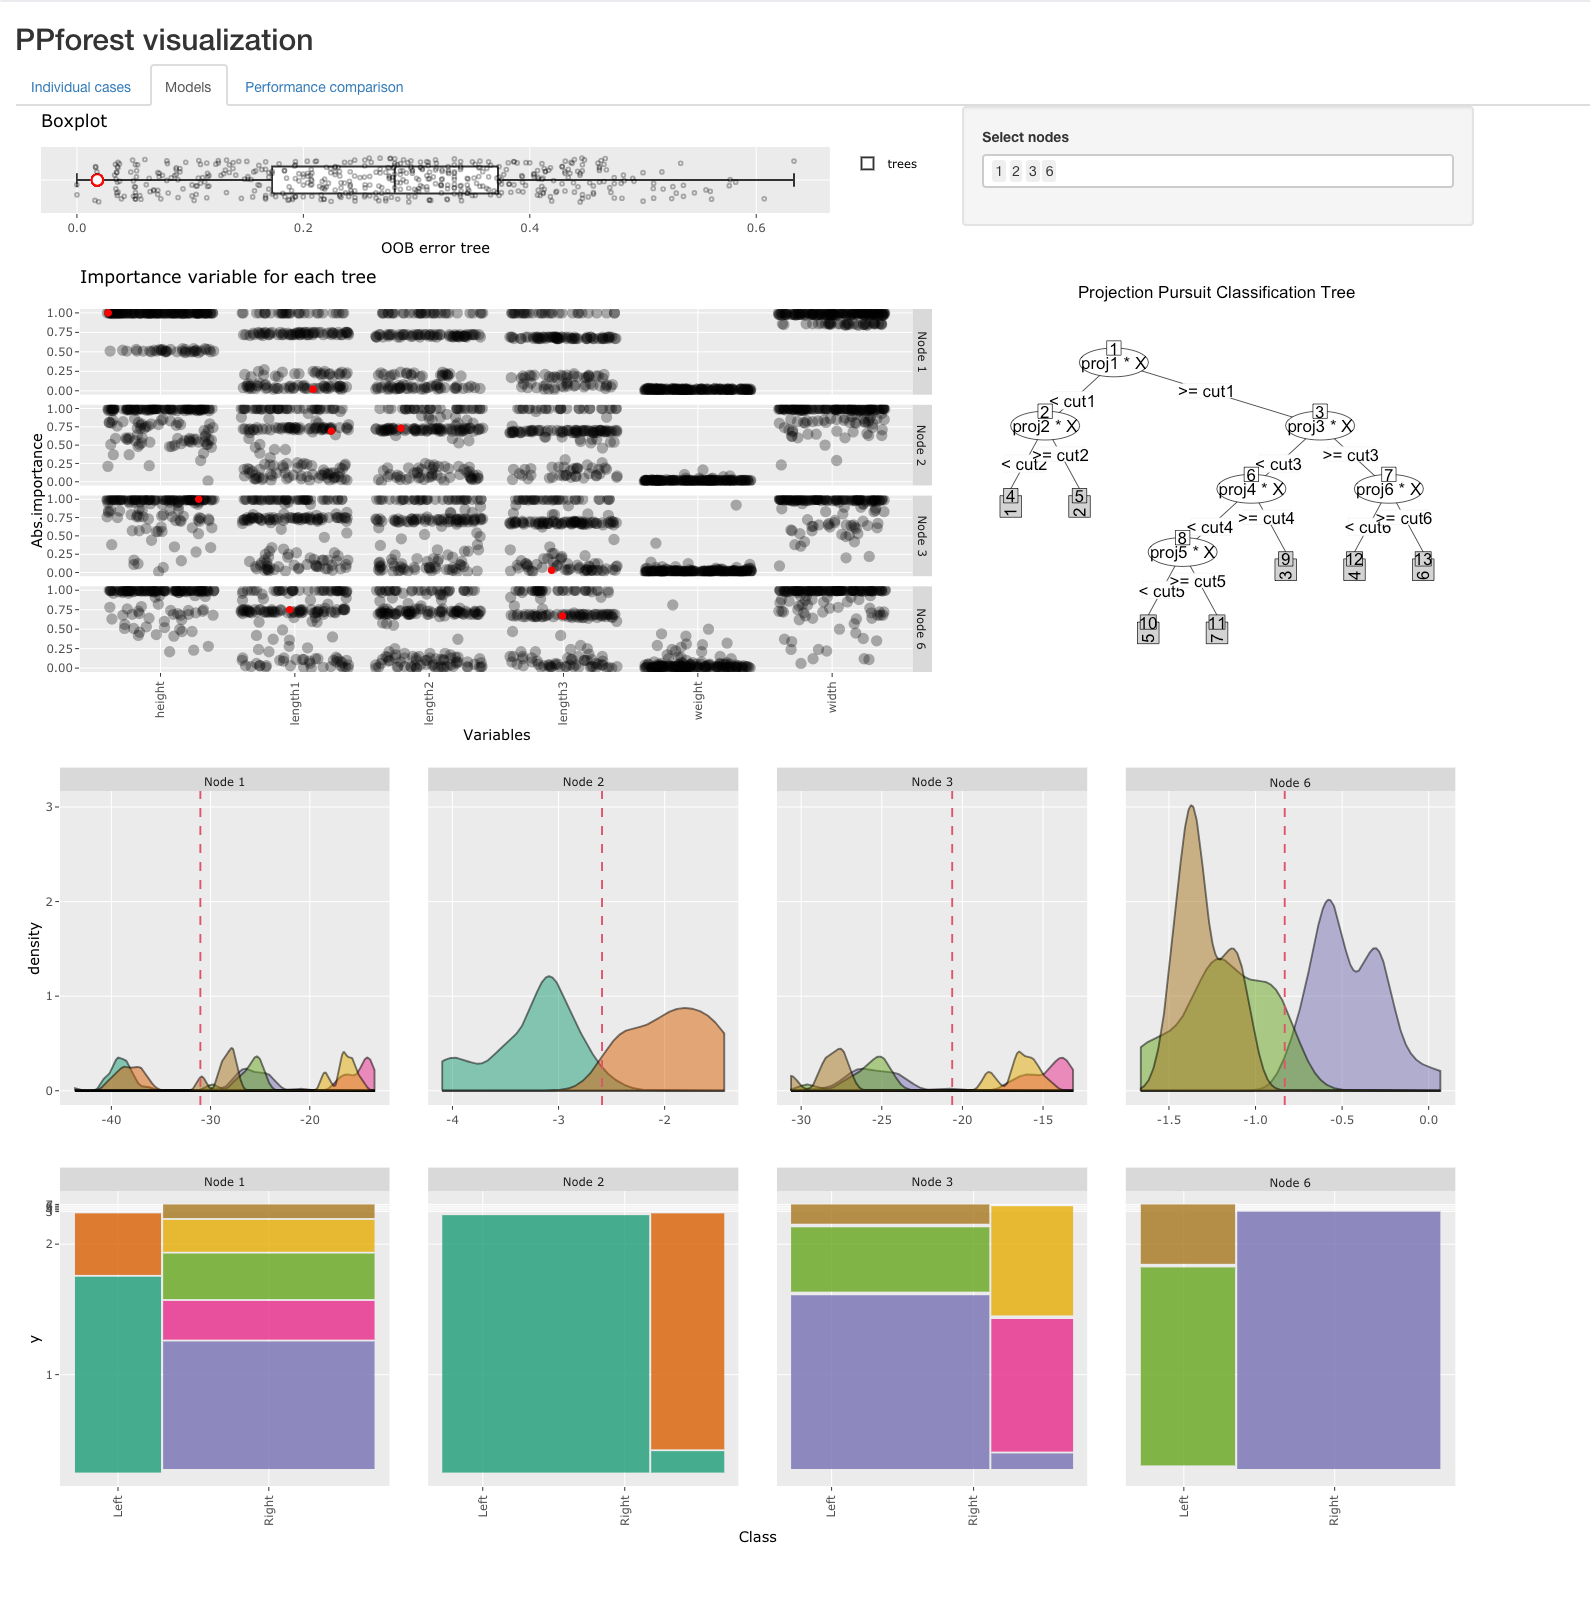
\includegraphics[width=1.1\linewidth]{tab2comp.png}
\caption{The individual model tab in the web app. The OOB error is displayed in a boxplot  including jittered points for all trees in the forest. Variable importance is displayed as jittered dot plots for selected nodes of all trees. The boxplot is linked to a display of the PPTree, the variable importance plot, and a density plot of the data projections showing splits at each selected node and confusion tables as mosaic plots. Clicking a point in the OOB error boxplot triggers various updates: each of the importance values for the same tree are highlighted (red), the tree that this corresponds to is drawn, the error for the tree is shown on the boxplot (in red), and the density plot and the mosaic plot are also updated. Also specific nodes can be selected to update the plots.  \label{tab2}}
\end{figure}


The diagram in Figure~\ref{tab2diag} illustrates the data pipeline for interactive graphics.
The data source is a \verb#PPforest# object. Interaction is driven in different ways, by the boxplot including jittered points. Selecting a point triggers a change in the data which cascades to re-draws of the other displays. Each plot has some information available on mouse over. Also selecting points in the variable importance triggers a change in the data and re-draws the displays corresponding to a specific tree. Finally selecting nodes update the data and re-draws the importance variable plot, density plot and mosaic plot.

\begin{figure}[hbpt]
\centering
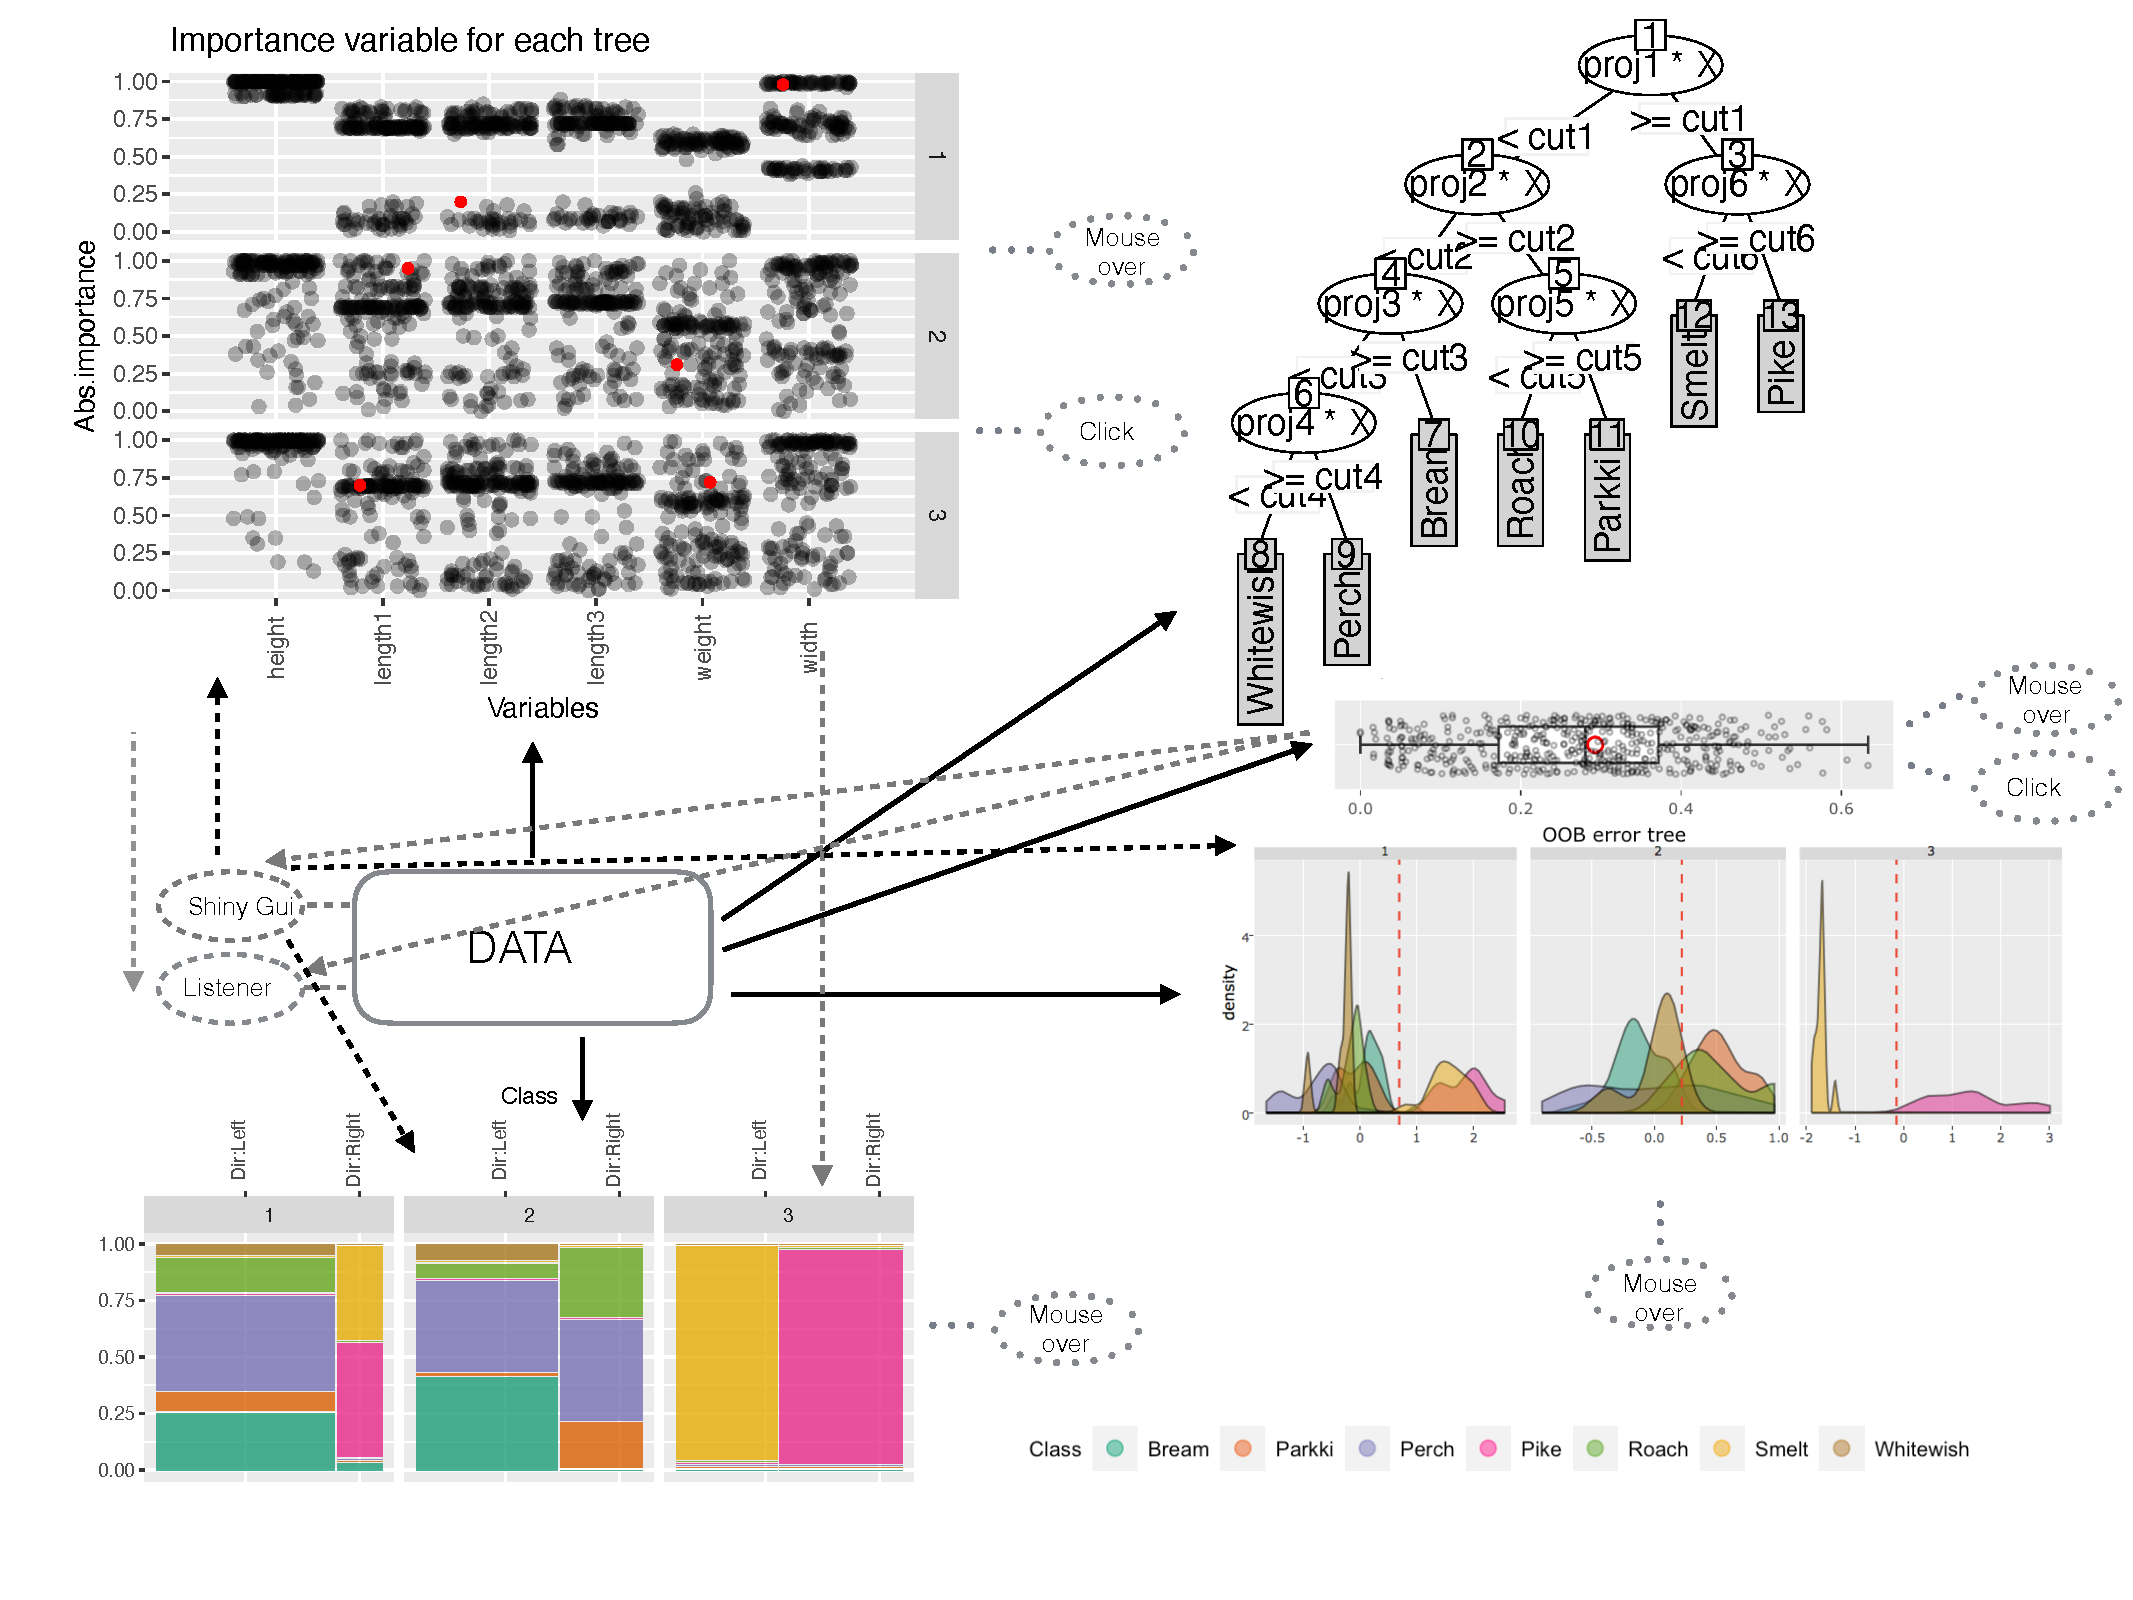
\includegraphics[width=1.05\linewidth]{fishT2.pdf}
\caption{Schematic diagram illustrating the interactivity in and between plots for model level exploration panel of the web app. The boxplot and the dotplot of variable importance has click selection, which invokes changes of the corresponding displays. Selecting a point in the boxplot update the node tree information (Shiny Gui) and update all the plots for the three first nodes, also nodes can be selected and update the corresponding plots. Finally selecting a point in the importance variable plot makes a change in the data, which propagates the importance values for other variables in this tree to be highlighted (red), draws the tree, highlights the error value of the tree, and shows the projections and confusion matrix for the three top nodes.}
\label{tab2diag}
\end{figure}
\newpage

\subsection{Performance Comparison}
The third tab (Figure \ref{tab3}) examines the PPF fit and compares the result with a RF fit. There are four displays for each type of model: (1) Variable importance for all trees in the forest (same as in the models tab), (2) a receiver operating characteristic curve (ROC) comparing sensitivity and specificity for each class, (3) OOB error by the number of trees to assess complexity, (4) overall variable importance. There is very little interaction on this tab. Users can select to focus on a subset of classes or choose the importance measure to show. Being able to focus on class can help to better understand how well the model performs across classes and the focus can be especially useful for unbalanced data. Examining the OOB error by trees enables an assessment of how few trees might be used to provide an equally accurate prediction of future data.

 The  ROC is used to summarize the trade-off between sensitivity and specificity. The plot shows the sensitivity and specificity when a parameter of the classifier is varied \citep{trevor2011elements}. The specificity and sensitivity were computed with the \verb#pROC# package.
 If more than two classes are available a multi-class ROC analysis is needed. Several solutions have been proposed for multi-class ROC. Some of the proposed reduced the multi-class problem to a set of binary problems. 
The approach used for a multi-class ROC analysis in this article is called one-against-all \citep{allwein2000reducing}.

\begin{figure}[hbpt]
\includegraphics[width=1\linewidth]{fish31.png}
\caption{Performance comparison tab of the web app. ROC curves displaying sensitivity against specificity for the classes are shown, along with the OOB error by the number of trees used to build the forest, and overall variable importance. Displays are shown for the PPF and RF, for comparison purposes. Users can select a class to focus on, using the text entry box. \label{tab3}}
\end{figure}
\newpage

\section{Discussion}\label{fur}

Having better tools to open up black box models will provide a better understanding of the data, the model strengths and weaknesses, and how the model will perform on future data. This visualization app provides a selection of interactive plots to diagnose PPF models. This shell could be used to make an app for other ensemble classifiers. The philosophy underlying the collection of displays is ``show the model in the data space''  explained in \citet{wickham2015visualizing}. It is not easy to do this, and to completely take this on would require plotting the model in the $p$-dimensional data space. In the simplest approach, as taken here, it means to link the model diagnostics to displays of the data. Then it is possible to probe and query to obtain a better understanding such as finding regions in the data that prove difficult to fit, and detract from the predictive accuracy, or that don't adhere to model assumptions.

The app is implemented using the technology for interactive graphics provided by the \verb# plotly# package. It was one of the first to experiment with the application of these tools. One challenge with plotly is that  when layers containing different data are created in a ggplot2, it is difficult to specify the unique keys required for linking with other plots.

There are some limitations with providing functionality through the app, and generally with the displays provided. Successful apps make it easier for the user to do common tasks, and this is the design principal here. Only limited functionality is provided to the user, but the code is available and a knowledgeable data analyst might use this as a basis for extending the methods as appropriate for their data. Performance of the app is good for relatively small data sets. If the number of observations is large, overploting will be an issue in some of the visualizations. If the number of variables is large, the parallel coordinate plot and plot of variable importance would benefit by the addition of a user input to select variables.

There are many possible extensions to the app that could help it to be a tool for model refinement:

\begin{enumerate}
\item Using the diagnostics to weed out under-performing models in the ensemble.
\item Identifying and boosting models that perform well, particularly if they do well for problematic subsets of the data.
\item Problematic cases could be removed, and ensembles re-fit.
\item Classes as a whole could be aggregated or re-organised as suggested by the model diagnostics, to produce a more effective hierarchical approach to the multiple class problem.
\end{enumerate}
\noindent Working within the R environment makes all of these possible when using command line outside the app, given that the unique IDs of models and cases can be exported from the app.

The app has helped to identify ways to improve the PPtree algorithm and consequently, the PPF model which especially apply to multiclass problems. Multiple splits for the same class would enable nonlinear classifications. Split criteria tend to place boundaries too close to some groups, due to heteroskedasticity being induced by aggregating classes. Forests are not always better than their constituent trees, and if the trees can be built better, the forest will provide better predictions.

\section{Supplementary Materials}
This article was written with the R packages knitr \citep{xie:2015}, ggplot2 \citep{hadley:2009}, and dplyr \citep{dplyr}, and the files to reproduce the article and results is available at https://github.com/natydasilva/PPforestViz. The code to reproduce the shiny app is available at https://github.com/natydasilva/shinyPPforest.


\bibliographystyle{apalike}
\bibliography{ppforestpaperbib}
\end{document}
